\clearpage
\section{Explaining V1 Receptive Field Formation}

\subsection{Code organization}

The code organization is similar as in the question $1.2$. The files description
is given below.
\begin{itemize}
    \item \texttt{ODE.py} contains the abstract class \texttt{ODE} which defines
        the interface for ordinary differential equations.
    \item \texttt{Integrator.py} contains the abstract class \texttt{Integrator}
        and its derived classes \texttt{ForwardDifference} and
        \texttt{RungeKutta4} which numerically solve an ordinary differential
        equation.
    \item \texttt{Neuron.py} contains the class \texttt{Neuron}, which derives
        from \texttt{ODE}. It implements the functionality of a BCM neuron, and
        also can be treated as an ODE.
    \item \texttt{Patch.py} contains the class \texttt{Patch} which holds the
        on and off arrays of an input patch.
    \item \texttt{preprocess.py} implements the functionality for preprocessing
        the given images and creation of the patches.
    \item \texttt{plotter.py} contains the various functionality for plotting.
    \item \texttt{simulation.py} loads the preprocessed data, generates the
        patches and runs the simulation. In the end, it stores generated plots
        in the directory \texttt{simulation}.
\end{itemize}

\subsection{Preprocessing}
Normalization and generation of input patches was done in a separate
preprocessing step. Preprocessing is called with
\begin{lstlisting}[language=bash]
$ python preprocess.py
\end{lstlisting}
Normalization step creates the file with suffix \texttt{\_normalized.data},
which contains a \texttt{numpy} array of normalized input image, serialized to
string. Afterwards, the file which describes patches is created. Its suffix is
\texttt{\_patches.data}. It contains $5000$ rows, where each row has the pixel
coordinates of upper-left corner of the $16\times16$ pixel patch. No two
patches are identical. This way of describing patches makes sure that additional
preprocessed data won't take too much memory, while still being easy to create
generated patches.

\subsection{Simulation}

\begin{figure}[h]
\centering
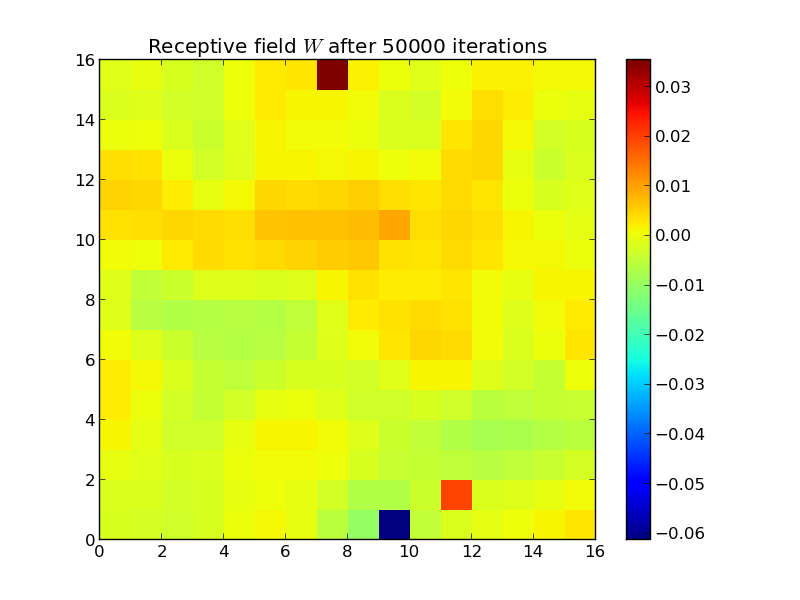
\includegraphics[width=0.7\textwidth]{../ex3/results1/img06}
\caption{Receptive field $W$ after $50000$ iterations. Some changes start to be
observable.}
\label{fig:img06}
\end{figure}

\begin{figure}[h]
\centering
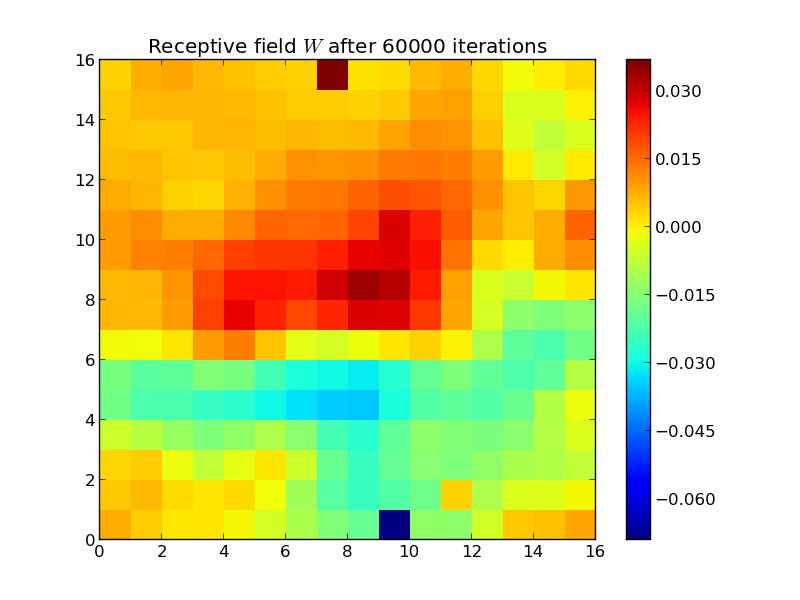
\includegraphics[width=0.7\textwidth]{../ex3/results1/img07}
\caption{Receptive field $W$ after $60000$ iterations. Positive and negative
weights start to separate}
\label{fig:img07}
\end{figure}

\begin{figure}[h]
\centering
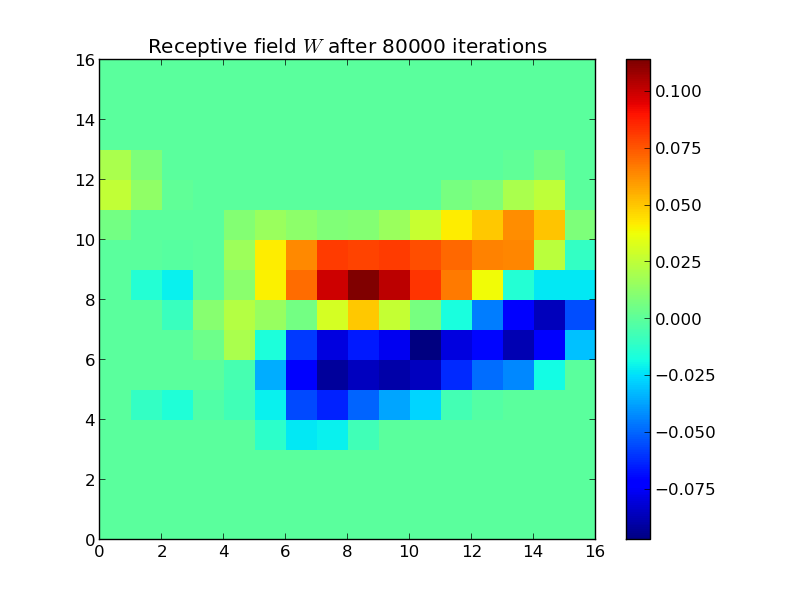
\includegraphics[width=0.7\textwidth]{../ex3/results1/img09}
\caption{Receptive field $W$ after $80000$ iterations. It is starting to look
like an edge detecting filter.}
\label{fig:img09}
\end{figure}

\begin{figure}[h]
\centering
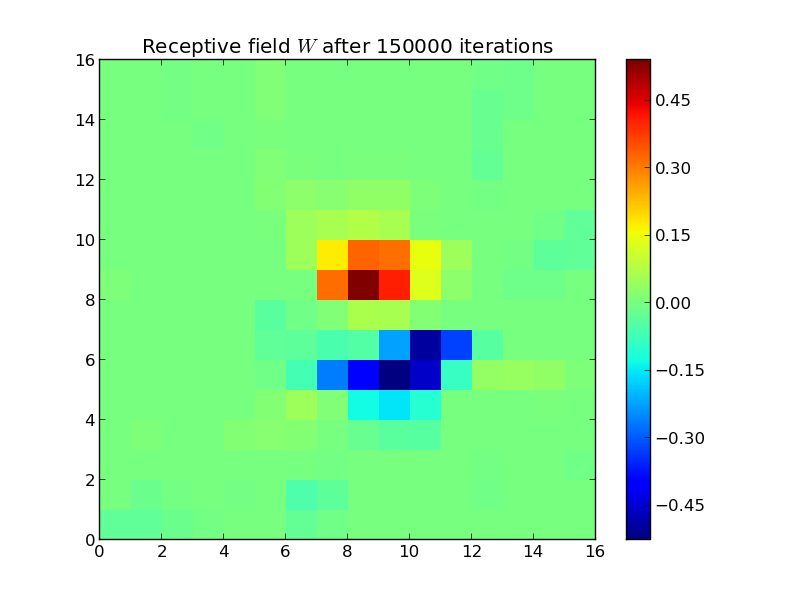
\includegraphics[width=0.7\textwidth]{../ex3/results1/img16}
\caption{Receptive field $W$ after $150000$ iterations. Filter didn't change
much after many iterations.}
\label{fig:img16}
\end{figure}

\begin{figure}[h]
\centering
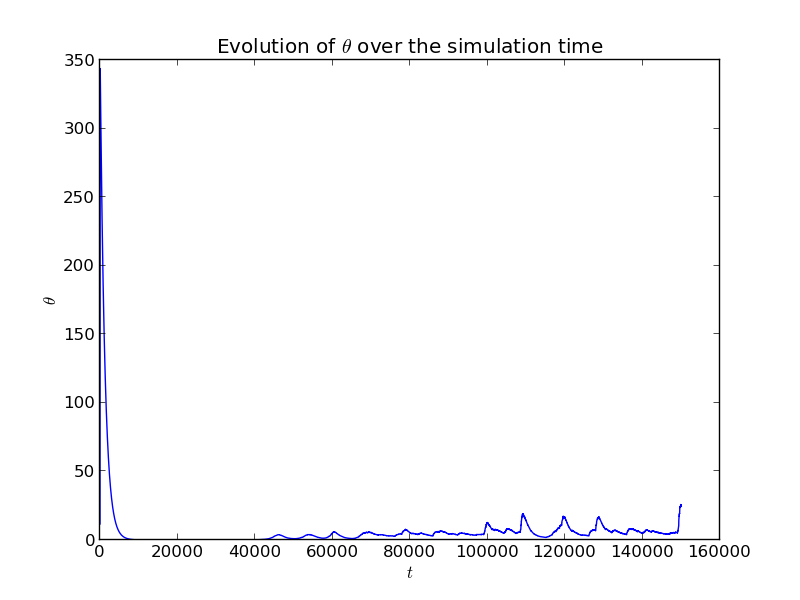
\includegraphics[width=0.7\textwidth]{../ex3/results1/theta}
\caption{Evolution of parameter $\theta$ during thesimulation. Starting peak
meant the bigger changes in $W$, but later everything stabilized.}
\label{fig:theta}
\end{figure}

The simulation was performed many times. Every simulation was done with $150000$
iterations, with $50000$ different patches. Every simulation has had different
permutations of patches, and occasionally, patches were constructed again using
preprocessing. Figures \ref{fig:img06}, \ref{fig:img07}, \ref{fig:img09} and
\ref{fig:img16} show the typical development of a receptive field. After the
random initialization, there is a period of learning where no particular
structure can be seen. It usually contains only intensities around the zero
value. After enough patches have been introduced to the neuron, it starts to
observe some lines or patterns. Soon after, a clear differentiation of positive
and negative weights can be observed, like in the Figure \ref{fig:img07}.
Afterwards, it converges to a field that resembles a Gabor filter, and stays
that way with only slight occasional changes, what can be observed from Figures
\ref{fig:img09} and \ref{fig:img16}.

It is worth noting that the orientation of the obtained Gabor filter is always
the same, regardless of the preprocessing or initialization. That implies that
this particular way of connecting the weights, combined with the BCM rule,
yields only one orientation of the filter.

In addition, Figure \ref{fig:theta} shows how the parameter $\theta$ evolves
during the simulation. It was observed that whenever $\theta$ adopts a larger
value, changes in the receptive field are more noticeable. Thus, it is expected
to have larger pikes of $\theta$ in the beginning of the simulation, which then
exponentially tends to zero with slight oscillations.

In conclusion, this simulation serves as an example that BCM learning rule can
be considered correct for the neurons in the primary visual cortex. When
presented a large amount of different patches, neuron will learn to separate
independent components and the result will be a receptive field which resembles
the Gabor filter.
